\chapter{Les bases}
    %\addcontentsline{toc}{chapter}{}

\section{Introduction}


\section{Écriture d'un paragraphe simple}

Les activités scientifiques d'un étudiant sont de nature à témoigner de son dévouement à la recherche scientifique et à l'innovation. Les candidats porteurs de projet seront favorisés par le fait qu'ils ont une activité prête à la mise en \oe uvre.


\subsection{Activités réalisées }
Le projet, à travers les formations spécifiques, sert à aider les étudiants à mettre en \oe uvre leurs projets. Les formations offertes constituent, en effet, des stages de perfectionnement pour des candidats déja initiés et ayant dans leurs actifs des formations suivies et des projets réalisés. 

\subsection{Lettre de motivation}
La lettre de motivation doit dégager les attentes du candidat de la formation ou des formations à suivre. La rédaction doit préciser la valeur ajoutée attendue de la participation. L'évaluation de la lettre tiendra compte de la qualité de la rédaction et la clarté des idées du candidat.
Cinq critères doivent être vérifiés pour qu'une lettre de motivation soit excellente.

\section{Insertion de figure}
%\\
\begin{figure}[h!]
	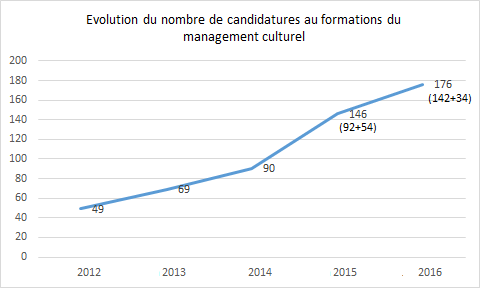
\includegraphics[width=13cm]{image3.png}
	\caption{Logo de l'entreprise SOPAL}
	\label{imag3}
\end{figure}


\section{Insertion d'un tableau}

L'attribution des points en fonction des activités culturelles du candidat est détaillée dans le tableau \ref{tab3}. 

\begin{table}
\begin{center}
\caption{Attribution des points en fonction du nombre de projets culturels réalisés}
\label{tab3}
\begin{tabular}{|l|l|}
\hline
\rowcolor[gray]{0.8}\bfseries Nombre de projets réalisés & \bfseries Points\\
\hline
>= 5 &40\\
\hline
=4 & 25\\
\hline
=3 & 15\\
\hline
=2 &10\\
\hline
=1 & 5\\
\hline
Autre & 0\\
\hline
\end{tabular}
\end{center}

\end{table}





L'attribution des points, à la lettre de motivation, en fonction du respect des critères sus mentionnés est détaillée dans le tableau \ref{tab5}.

\begin{table}
\begin{center}
\caption{Attribution des points à la lettre de motivation en fonction du nombre de critères respectés}
\label{tab5}
\begin{tabular}{|l|l|l|}
\hline
\rowcolor[gray]{0.8}\bfseries Respect des critères &\bfseries Évaluation &\bfseries Points \\
\hline
C1+C2+C3+C4+C5 & Excellente &18\\
\hline
C1+C2+C3+C4 & Très bien & 16\\
\hline
C1+C2+C3 & Bien & 14\\
\hline
C1+C2 & Moyen &10\\
\hline
C1 & Faible & 2\\
\hline
Autre & Insuffisant & 0\\
\hline
\end{tabular}
\end{center}

\end{table}



\section{Les listes}
\subsection{Les listes numérotées}

\begin{enumerate}

\item \textbf{C1}:La rédaction dans un langage soutenu sans erreurs d'orthographe et de grammaire,
\item \textbf{C2}:La rédaction avec des propos clairs et perspicaces,
\item \textbf{C3}:La lettre doit dégager l'intérêt de suivre la formation pour le candidat,
\item \textbf{C4}:Le candidat doit prouver son sérieux et son désir de participer à la formation, 
\item \textbf{C5}:La Lettre doit montrer l'impact positif que pourrait avoir la formation sur la concrétisation du projet du candidat.
\end{enumerate}

\subsection{Les listes non numérotées}

\begin{itemize}

\item \textbf{C1}:La rédaction dans un langage soutenu sans erreurs d'orthographe et de grammaire,
\item \textbf{C2}:La rédaction avec des propos clairs et perspicaces,
\item \textbf{C3}:La lettre doit dégager l'intérêt de suivre la formation pour le candidat,
\item \textbf{C4}:Le candidat doit prouver son sérieux et son désir de participer à la formation, 
\item \textbf{C5}:La Lettre doit montrer l'impact positif que pourrait avoir la formation sur la concrétisation du projet du candidat.
\end{itemize}

\section{Conclusion}
